
% LaTeX Beamer file automatically generated from DocOnce
% https://github.com/hplgit/doconce

%-------------------- begin beamer-specific preamble ----------------------

\documentclass{beamer}

\usetheme{red_shadow}
\usecolortheme{default}

% turn off the almost invisible, yet disturbing, navigation symbols:
\setbeamertemplate{navigation symbols}{}

% Examples on customization:
%\usecolortheme[named=RawSienna]{structure}
%\usetheme[height=7mm]{Rochester}
%\setbeamerfont{frametitle}{family=\rmfamily,shape=\itshape}
%\setbeamertemplate{items}[ball]
%\setbeamertemplate{blocks}[rounded][shadow=true]
%\useoutertheme{infolines}
%
%\usefonttheme{}
%\useinntertheme{}
%
%\setbeameroption{show notes}
%\setbeameroption{show notes on second screen=right}

% fine for B/W printing:
%\usecolortheme{seahorse}

\usepackage{pgf}
\usepackage{graphicx}
\usepackage{epsfig}
\usepackage{relsize}

\usepackage{fancybox}  % make sure fancybox is loaded before fancyvrb

\usepackage{fancyvrb}
\usepackage{minted} % requires pygments and latex -shell-escape filename
%\usepackage{anslistings}
%\usepackage{listingsutf8}

\usepackage{amsmath,amssymb,bm}
%\usepackage[latin1]{inputenc}
\usepackage[T1]{fontenc}
\usepackage[utf8]{inputenc}
\usepackage{colortbl}
\usepackage[english]{babel}
\usepackage{tikz}
\usepackage{framed}
% Use some nice templates
\beamertemplatetransparentcovereddynamic

% --- begin table of contents based on sections ---
% Delete this, if you do not want the table of contents to pop up at
% the beginning of each section:
% (Only section headings can enter the table of contents in Beamer
% slides generated from DocOnce source, while subsections are used
% for the title in ordinary slides.)
\AtBeginSection[]
{
  \begin{frame}<beamer>[plain]
  \frametitle{}
  %\frametitle{Outline}
  \tableofcontents[currentsection]
  \end{frame}
}
% --- end table of contents based on sections ---

% If you wish to uncover everything in a step-wise fashion, uncomment
% the following command:

%\beamerdefaultoverlayspecification{<+->}

\newcommand{\shortinlinecomment}[3]{\note{\textbf{#1}: #2}}
\newcommand{\longinlinecomment}[3]{\shortinlinecomment{#1}{#2}{#3}}

\definecolor{linkcolor}{rgb}{0,0,0.4}
\hypersetup{
    colorlinks=true,
    linkcolor=linkcolor,
    urlcolor=linkcolor,
    pdfmenubar=true,
    pdftoolbar=true,
    bookmarksdepth=3
    }
\setlength{\parskip}{7pt}  % {1em}

\newenvironment{doconceexercise}{}{}
\newcounter{doconceexercisecounter}
\newenvironment{doconce:movie}{}{}
\newcounter{doconce:movie:counter}

\newcommand{\subex}[1]{\noindent\textbf{#1}}  % for subexercises: a), b), etc

%-------------------- end beamer-specific preamble ----------------------

% Add user's preamble




% insert custom LaTeX commands...

\raggedbottom
\makeindex

%-------------------- end preamble ----------------------

\begin{document}

% matching end for #ifdef PREAMBLE
% #endif

\newcommand{\half}{\frac{1}{2}}
\newcommand{\halfi}{{1/2}}
\newcommand{\tp}{\thinspace .}

\newcommand{\uex}{{u_{\small\mbox{e}}}}
\newcommand{\uexd}[1]{{u_{\small\mbox{e}, #1}}}
\newcommand{\vex}{{v_{\small\mbox{e}}}}
\newcommand{\vexd}[1]{{v_{\small\mbox{e}, #1}}}
\newcommand{\Aex}{{A_{\small\mbox{e}}}}

% Operators
\newcommand{\Ddt}[1]{\frac{D #1}{dt}}
\newcommand{\E}[1]{\hbox{E}\lbrack #1 \rbrack}
\newcommand{\Var}[1]{\hbox{Var}\lbrack #1 \rbrack}
\newcommand{\Std}[1]{\hbox{Std}\lbrack #1 \rbrack}

\newcommand{\xpoint}{\bm{x}}
\newcommand{\normalvec}{\bm{n}}
\newcommand{\Oof}[1]{\mathcal{O}(#1)}

% Boldface vectors/tensors
\newcommand{\x}{\bm{x}}
\newcommand{\X}{\bm{X}}
\renewcommand{\u}{\bm{u}}
\renewcommand{\v}{\bm{v}}
\newcommand{\w}{\bm{w}}
\newcommand{\acc}{\bm{a}}
\newcommand{\rpos}{\bm{r}}
\newcommand{\V}{\bm{V}}
\newcommand{\e}{\bm{e}}
\newcommand{\f}{\bm{f}}
\newcommand{\F}{\bm{F}}
\newcommand{\stress}{\bm{\sigma}}
\newcommand{\strain}{\bm{\varepsilon}}
\newcommand{\stressc}{{\sigma}}
\newcommand{\strainc}{{\varepsilon}}
\newcommand{\I}{\bm{I}}
\newcommand{\T}{\bm{T}}

\newcommand{\dfc}{\alpha}  % diffusion coefficient
% Unit vectors
\newcommand{\ii}{\bm{i}}
\newcommand{\jj}{\bm{j}}
\newcommand{\kk}{\bm{k}}
\newcommand{\ir}{\bm{i}_r}
\newcommand{\ith}{\bm{i}_{\theta}}
\newcommand{\iz}{\bm{i}_z}

% Index sets
\newcommand{\Ix}{\mathcal{I}_x}
\newcommand{\Iy}{\mathcal{I}_y}
\newcommand{\Iz}{\mathcal{I}_z}
\newcommand{\It}{\mathcal{I}_t}
%\newcommand{\Ix}{{I_x}}
%\newcommand{\Iy}{{I_y}}
%\newcommand{\Iz}{{I_z}}
%\newcommand{\It}{{I_t}}
%\newcommand{\If}{\mathcal{I}}     % for FEM
\newcommand{\If}{\mathcal{I}_s}     % for FEM
%\newcommand{\If}{{I}}     % for FEM
%\newcommand{\Ifd}{\mathcal{I}_d}  % for FEM
\newcommand{\Ifd}{{I_d}}  % for FEM
\newcommand{\Ifb}{{I_b}}  % for FEM
\newcommand{\setb}[1]{#1^0}    % set begin
\newcommand{\sete}[1]{#1^{-1}} % set end
%\newcommand{\setl}[1]{#1\setminus\{\set1{#1}\}}
%\newcommand{\setr}[1]{#1\setminus\{\set0{#1}\}}
%\newcommand{\seti}[1]{#1\setminus\{\set0{#1},\set1{#1}\}}
\newcommand{\setl}[1]{#1^-}
\newcommand{\setr}[1]{#1^+}
\newcommand{\seti}[1]{#1^i}
\newcommand{\sequencei}[1]{\left\{ {#1}_i \right\}_{i\in\If}}

% Finite elements
\newcommand{\basphi}{\varphi}
\newcommand{\baspsi}{\psi}
\newcommand{\refphi}{\tilde\basphi}
\newcommand{\psib}{\bm{\psi}}
\newcommand{\sinL}[1]{\sin\left((#1+1)\pi\frac{x}{L}\right)}
\newcommand{\xno}[1]{x_{#1}}
%\newcommand{\xno}[1]{x^{(#1)}}
\newcommand{\Xno}[1]{X_{(#1)}}
\newcommand{\yno}[1]{y_{#1}}
\newcommand{\Yno}[1]{Y_{(#1)}}
\newcommand{\xdno}[1]{\bm{x}_{#1}}

% FEniCS commands
\newcommand{\dX}{\, \mathrm{d}X}
\newcommand{\dx}{\, \mathrm{d}x}
\newcommand{\ds}{\, \mathrm{d}s}
\newcommand{\Real}{\mathbb{R}}
\newcommand{\Integerp}{\mathbb{N}}
\newcommand{\Integer}{\mathbb{Z}}



% ------------------- main content ----------------------



% ----------------- title -------------------------

\title{Study guide: Analysis of exponential decay models}

% ----------------- author(s) -------------------------

\author{Hans Petter Langtangen\inst{1,2}}
\institute{Center for Biomedical Computing, Simula Research Laboratory\inst{1}
\and
Department of Informatics, University of Oslo\inst{2}}
% ----------------- end author(s) -------------------------

\date{Oct 10, 2015
% <optional titlepage figure>
% <optional copyright>
}

\begin{frame}[plain,fragile]
\titlepage
\end{frame}

\section{Analysis of finite difference equations}

\begin{frame}[plain,fragile]
\frametitle{Analysis of finite difference equations}

\label{decay:analysis}

Model:
\begin{equation}
u'(t) = -au(t),\quad u(0)=I
\end{equation}

Method:
\begin{equation}
u^{n+1} = \frac{1 - (1-\theta) a\Delta t}{1 + \theta a\Delta t}u^n
\label{decay:analysis:scheme}
\end{equation}

\begin{block}{Problem setting }
How good is this method? Is it safe to use it?
\end{block}


\end{frame}

\begin{frame}[plain,fragile]
\frametitle{Encouraging numerical solutions}

$I=1$, $a=2$, $\theta =1,0.5, 0$, $\Delta t=1.25, 0.75, 0.5, 0.1$.



% inline figure
\centerline{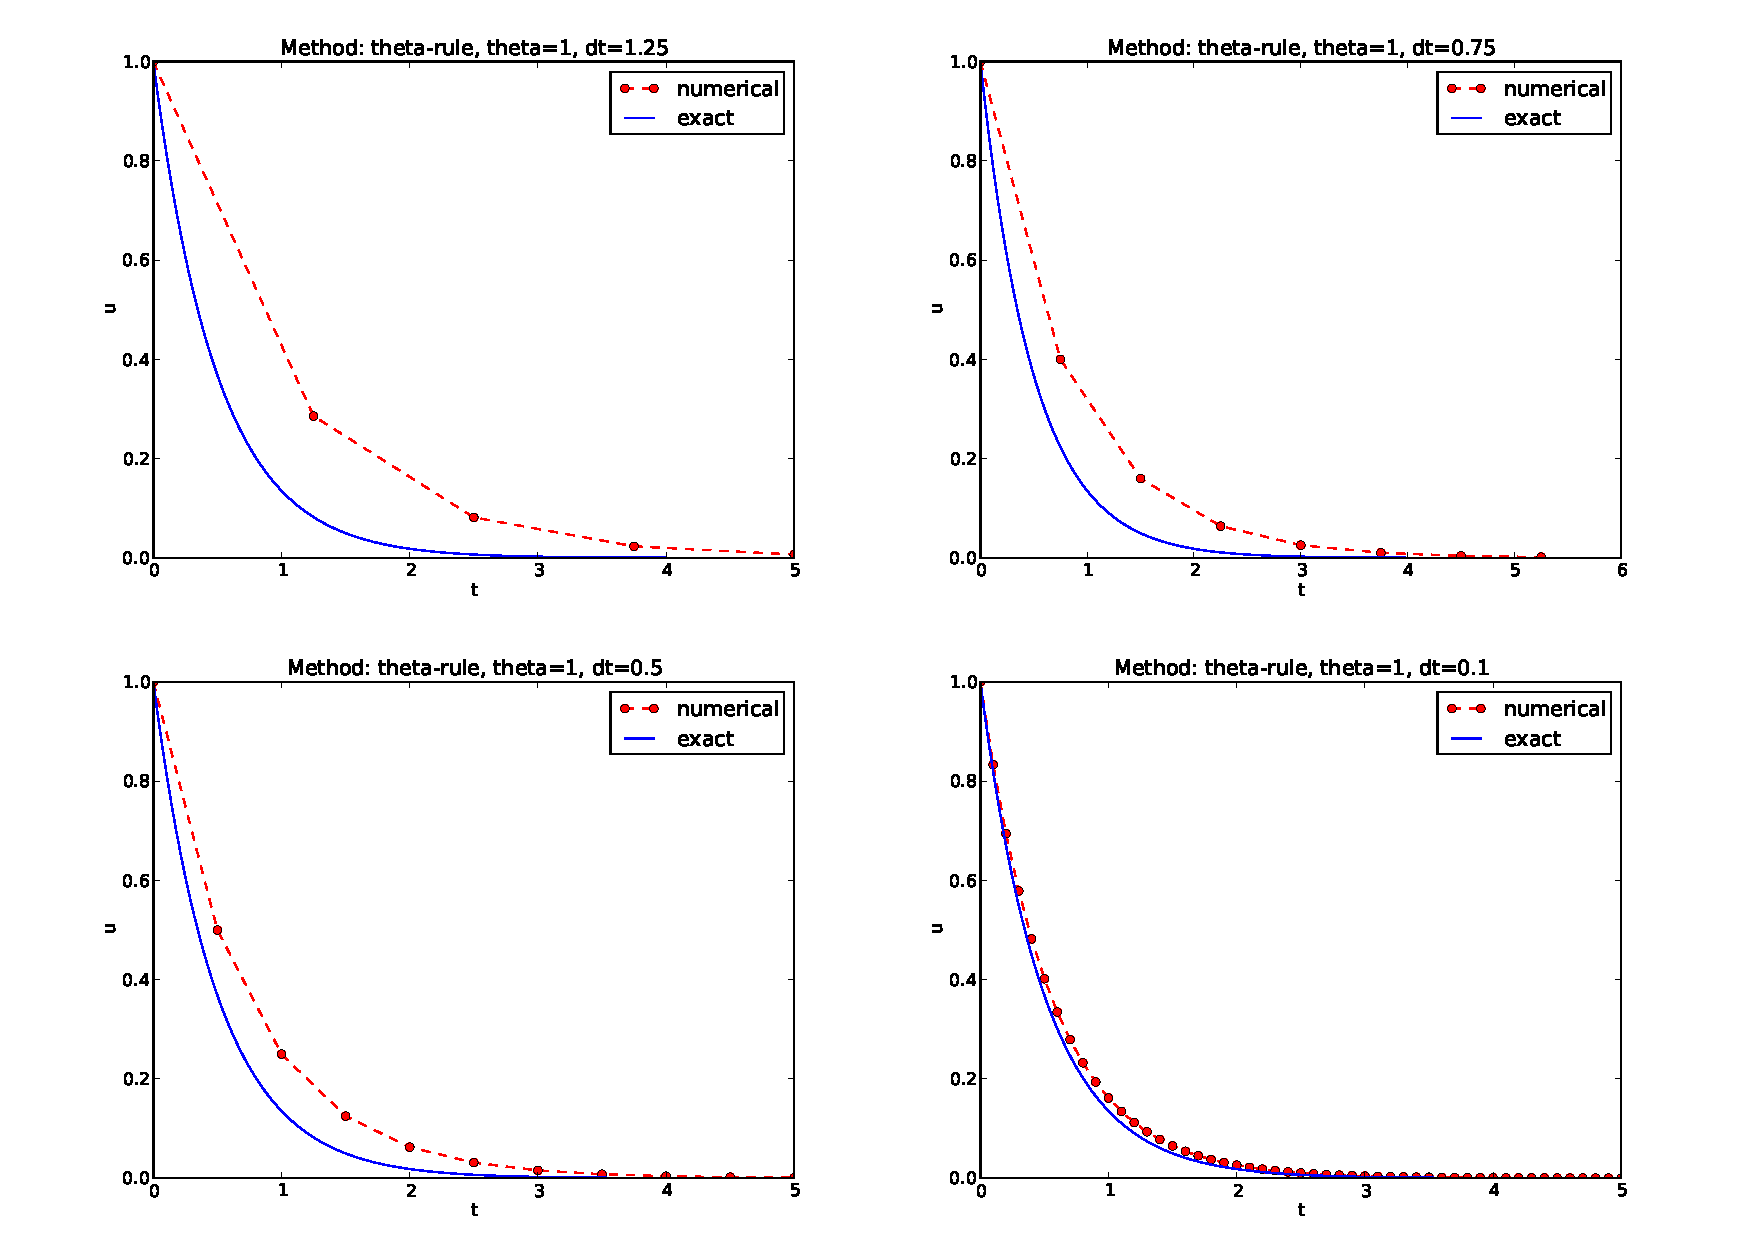
\includegraphics[width=1.1\linewidth]{fig-analysis/BE4c.pdf}}
\end{frame}

\begin{frame}[plain,fragile]
\frametitle{Discouraging numerical solutions; Crank-Nicolson}

% inline figure
\centerline{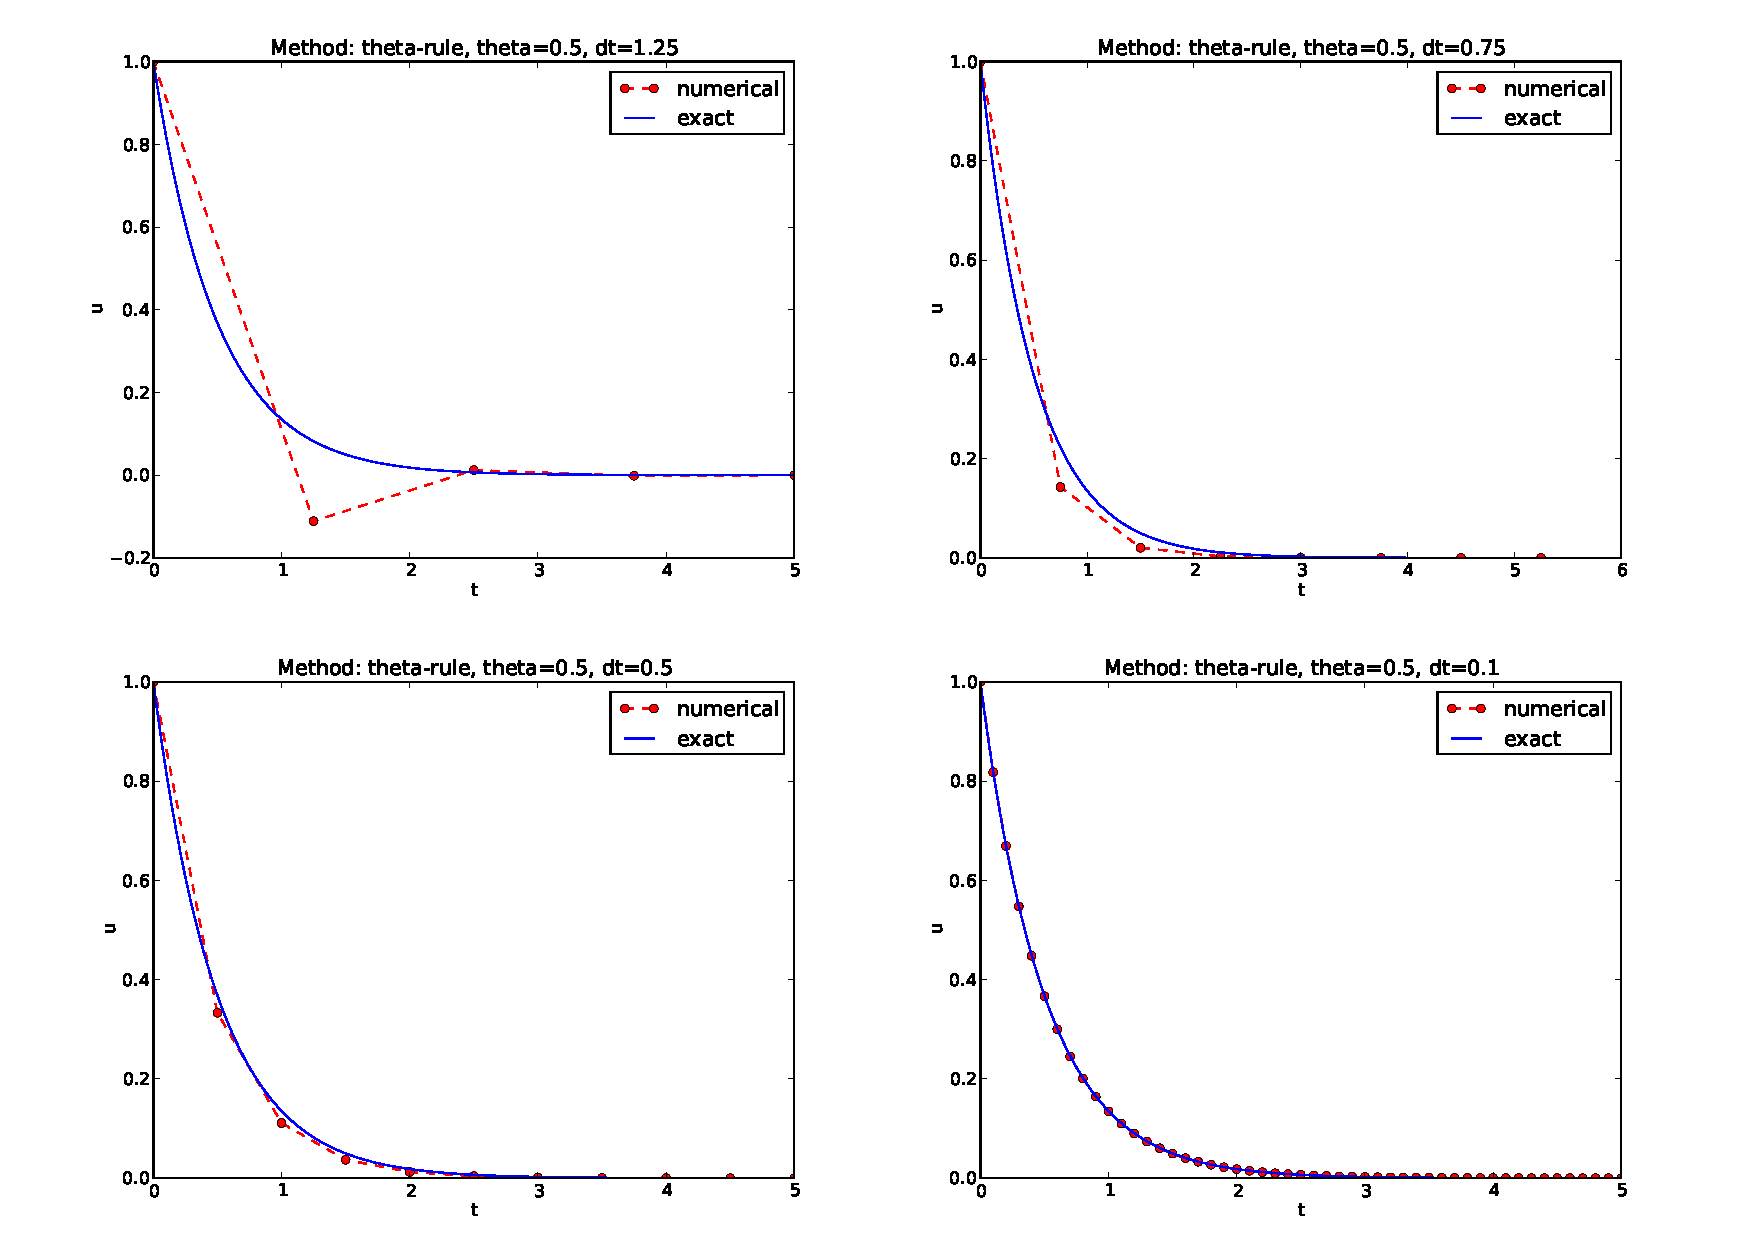
\includegraphics[width=1.1\linewidth]{fig-analysis/CN4c.pdf}}
\end{frame}

\begin{frame}[plain,fragile]
\frametitle{Discouraging numerical solutions; Forward Euler}

% inline figure
\centerline{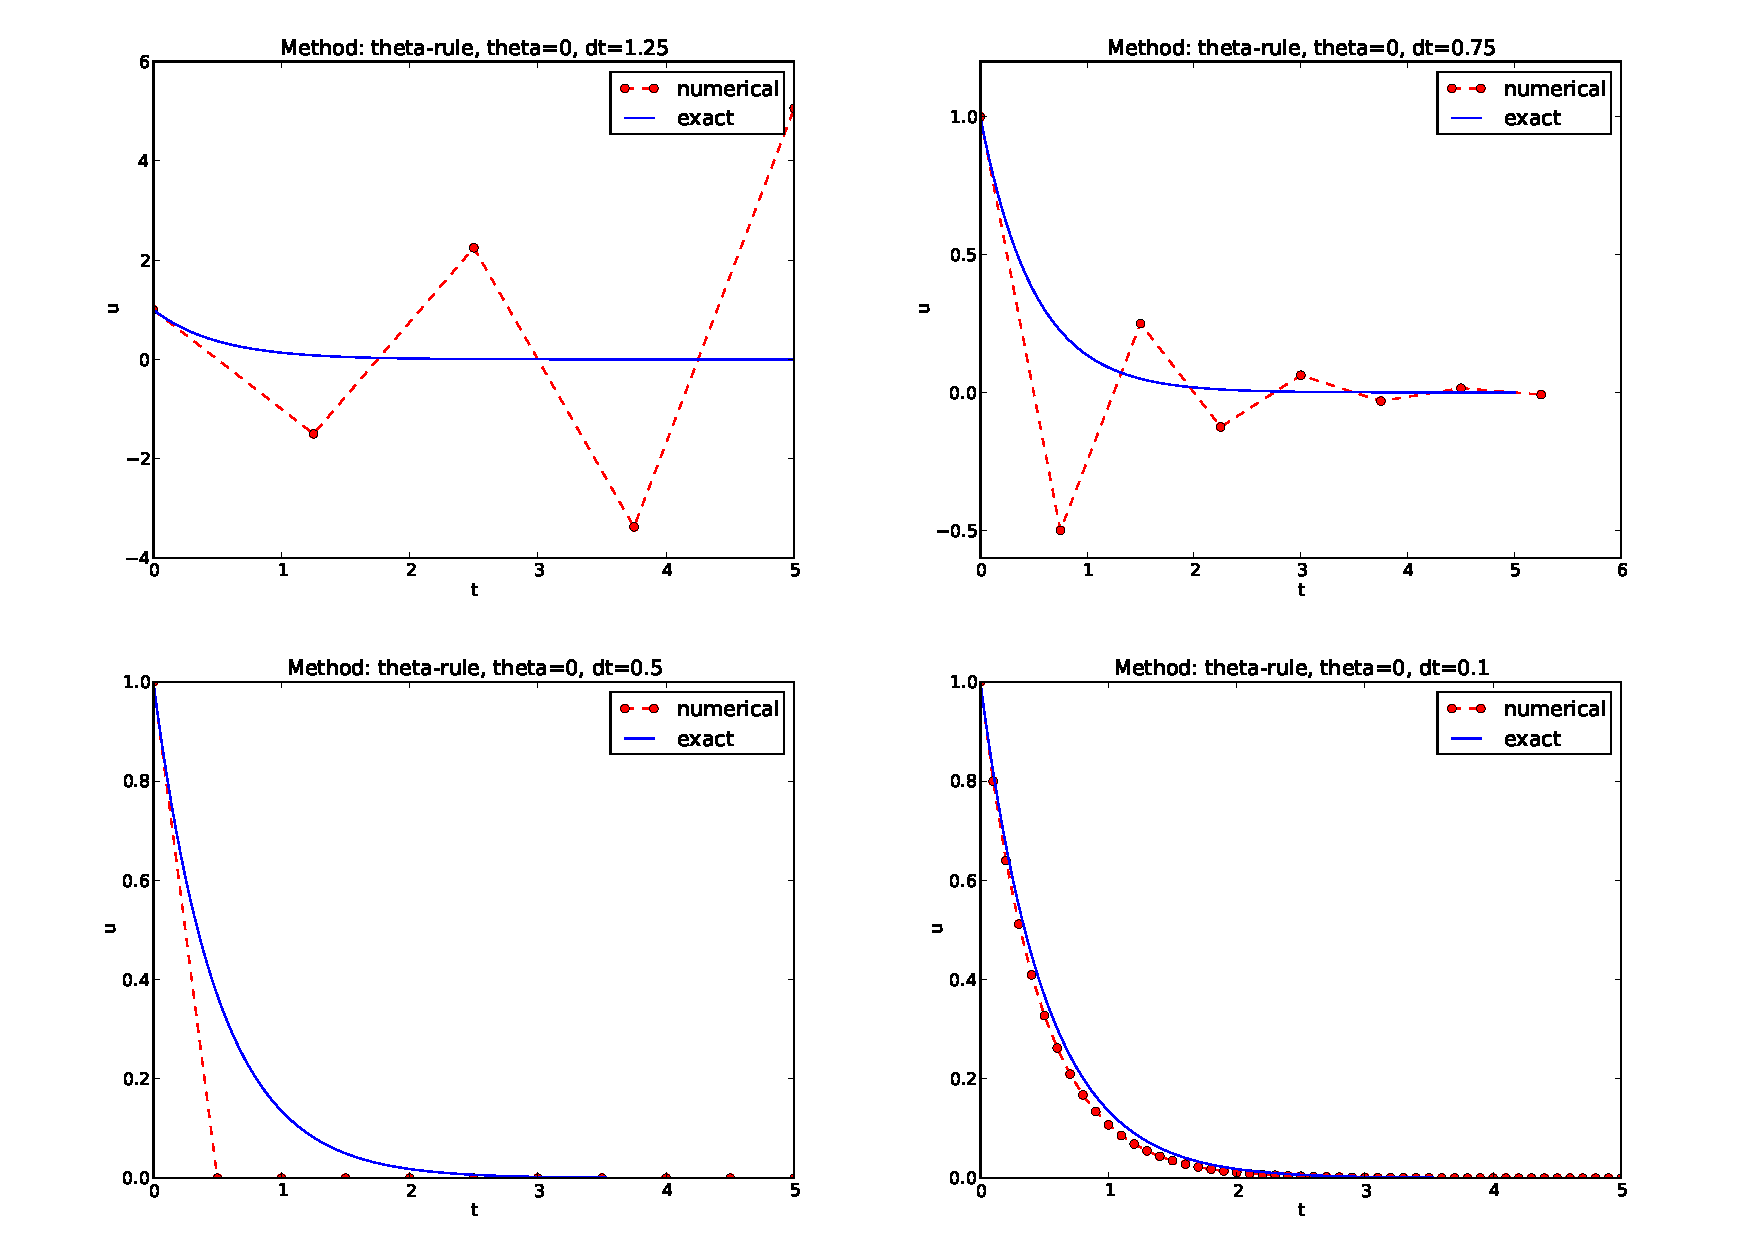
\includegraphics[width=1.1\linewidth]{fig-analysis/FE4c.pdf}}
\end{frame}

\begin{frame}[plain,fragile]
\frametitle{Summary of observations}

The characteristics of the displayed curves can be summarized as follows:

\begin{itemize}
  \item The Backward Euler scheme \emph{always} gives a monotone solution, lying above
    the exact curve.

  \item The Crank-Nicolson scheme gives the most accurate results, but for
    $\Delta t=1.25$ the solution oscillates.

  \item The Forward Euler scheme gives a growing, oscillating solution for
    $\Delta t=1.25$; a decaying, oscillating solution for $\Delta t=0.75$;
    a strange solution $u^n=0$ for $n\geq 1$ when $\Delta t=0.5$; and
    a solution seemingly as accurate as the one by the Backward Euler
    scheme for $\Delta t = 0.1$, but the curve lies \emph{below} the exact
    solution.
\end{itemize}

\noindent
\end{frame}

\begin{frame}[plain,fragile]
\frametitle{Problem setting}

\begin{block}{Goal }
We ask the question

\begin{itemize}
  \item Under what circumstances, i.e., values of
    the input data $I$, $a$, and $\Delta t$ will the Forward Euler and
    Crank-Nicolson schemes result in undesired oscillatory solutions?
\end{itemize}

\noindent
Techniques of investigation:

\begin{itemize}
 \item Numerical experiments

 \item Mathematical analysis
\end{itemize}

\noindent
Another question to be raised is

\begin{itemize}
 \item How does $\Delta t$ impact the error in the numerical solution?
\end{itemize}

\noindent
\end{block}
\end{frame}

\begin{frame}[plain,fragile]
\frametitle{Experimental investigation of oscillatory solutions}

The solution is oscillatory if
\[ u^{n} > u^{n-1}\]



% inline figure
\centerline{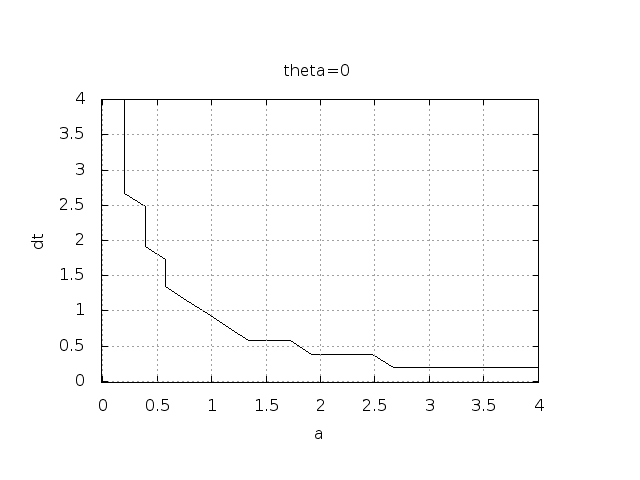
\includegraphics[width=0.9\linewidth]{fig-analysis/osc_region_FE.png}}



Seems that $a\Delta t < 1$ for FE and 2 for CN.
\end{frame}

\begin{frame}[plain,fragile]
\frametitle{Exact numerical solution}

Starting with $u^0=I$, the simple recursion (\ref{decay:analysis:scheme})
can be applied repeatedly $n$ times, with the result that

\begin{equation}
u^{n} = IA^n,\quad A = \frac{1 - (1-\theta) a\Delta t}{1 + \theta a\Delta t}
\label{decay:analysis:unex}
\end{equation}

Such an exact discrete solution is unusual, but very handy for analysis.
\end{frame}

\begin{frame}[plain,fragile]
\frametitle{Stability}

\index{stability}

Since $u^n\sim A^n$,

\begin{itemize}
 \item $A < 0$ gives a factor $(-1)^n$ and oscillatory solutions

 \item $|A|>1$ gives growing solutions

 \item Recall: the exact solution is \emph{monotone} and \emph{decaying}

 \item If these qualitative properties are not met, we say that the
   numerical solution is \emph{unstable}
\end{itemize}

\noindent
\end{frame}

\begin{frame}[plain,fragile]
\frametitle{Computation of stability in this problem}

$A < 0$ if

\[
\frac{1 - (1-\theta) a\Delta t}{1 + \theta a\Delta t} < 0
\]
To avoid oscillatory solutions we must have $A> 0$ and

\begin{equation}
\Delta t < \frac{1}{(1-\theta)a}\ 
\end{equation}

\begin{itemize}
 \item Always fulfilled for Backward Euler

 \item $\Delta t \leq 1/a$ for Forward Euler

 \item $\Delta t \leq 2/a$ for Crank-Nicolson
\end{itemize}

\noindent
\end{frame}

\begin{frame}[plain,fragile]
\frametitle{Computation of stability in this problem}

$|A|\leq 1$ means $-1\leq A\leq 1$

\begin{equation}
-1\leq\frac{1 - (1-\theta) a\Delta t}{1 + \theta a\Delta t} \leq 1
\label{decay:th:stability}
\end{equation}
$-1$ is the critical limit:

\begin{align*}
\Delta t &\leq \frac{2}{(1-2\theta)a},\quad \theta < \half\\ 
\Delta t &\geq \frac{2}{(1-2\theta)a},\quad \theta > {\half}
\end{align*}

\begin{itemize}
 \item Always fulfilled for Backward Euler and Crank-Nicolson

 \item $\Delta t \leq 2/a$ for Forward Euler
\end{itemize}

\noindent
\end{frame}

\begin{frame}[plain,fragile]
\frametitle{Explanation of problems with Forward Euler}

% inline figure
\centerline{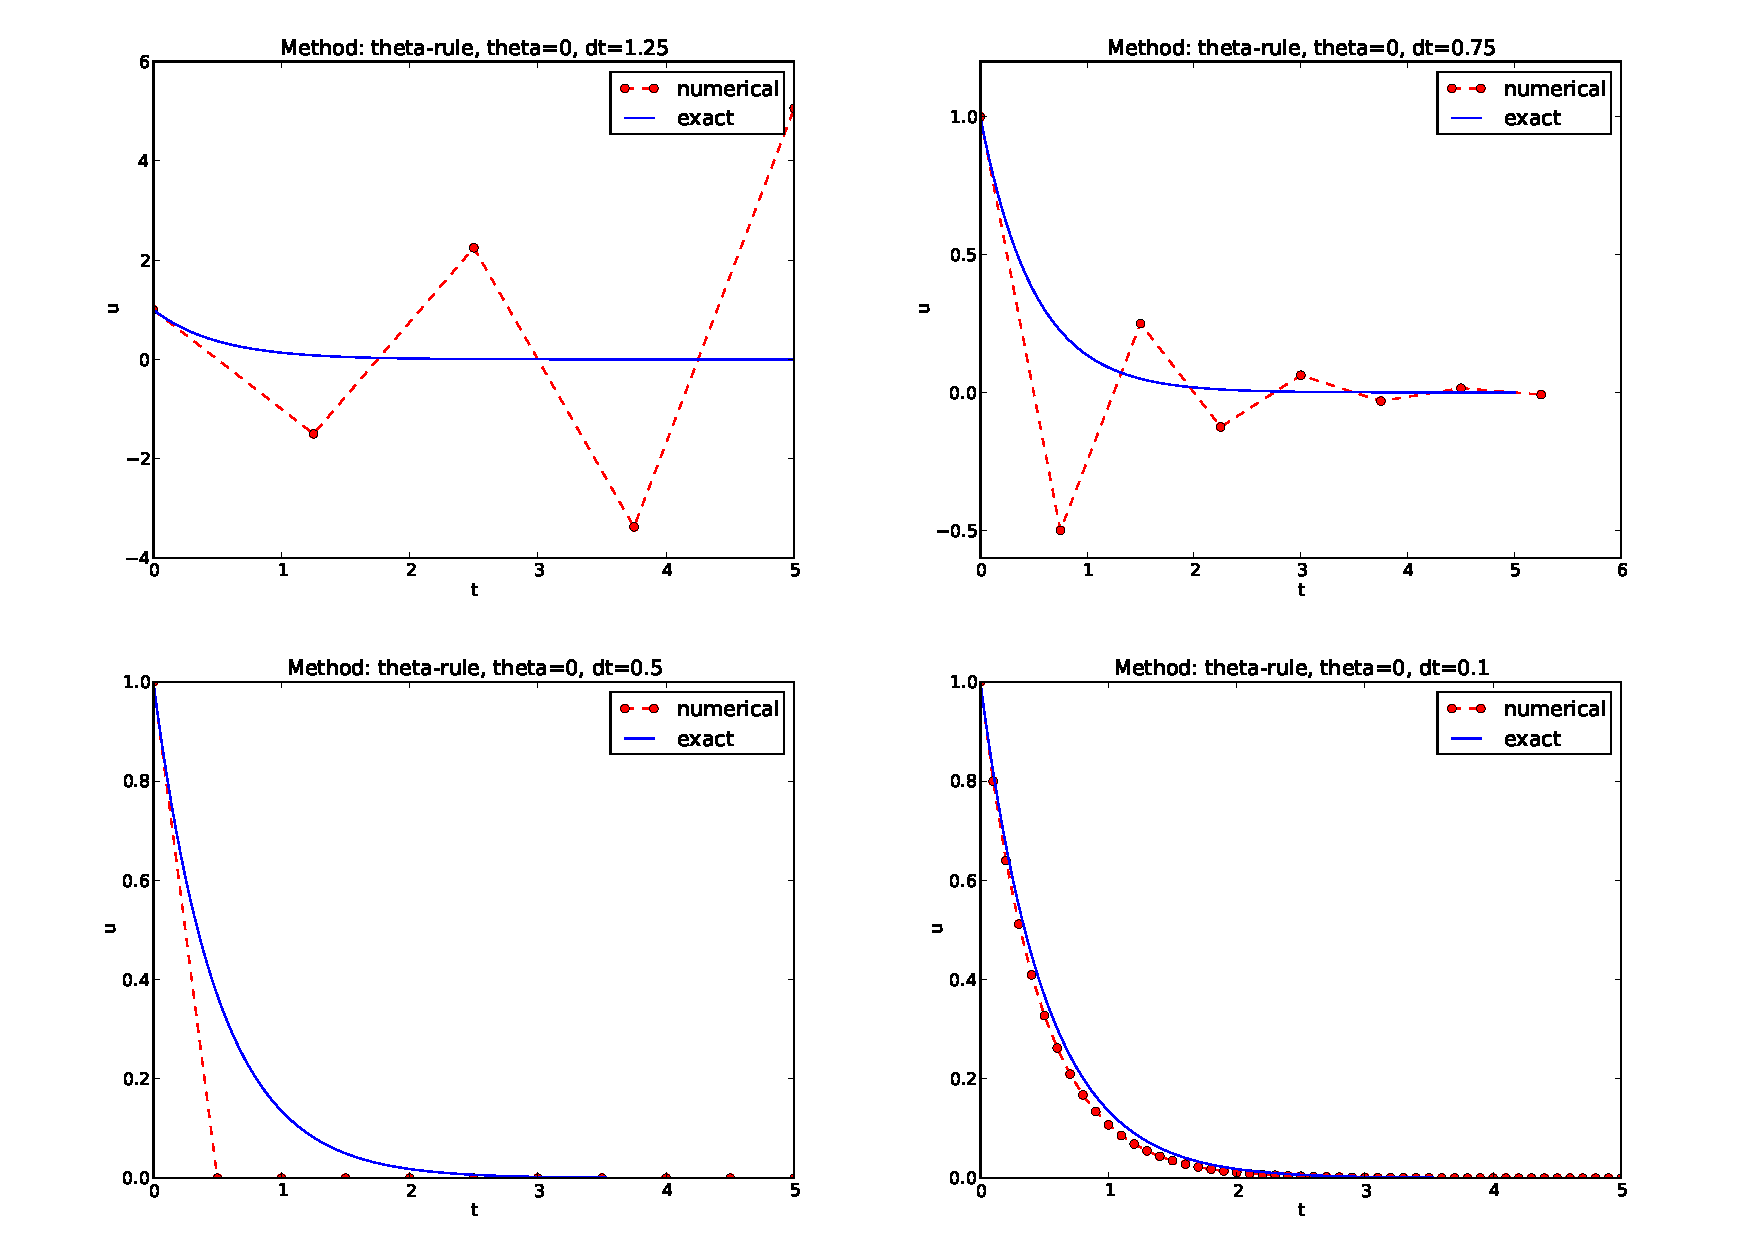
\includegraphics[width=1.1\linewidth]{fig-analysis/FE4c.pdf}}



\begin{itemize}
 \item $a\Delta t= 2\cdot 1.25=2.5$ and $A=-1.5$: oscillations and growth

 \item $a\Delta t = 2\cdot 0.75=1.5$ and $A=-0.5$: oscillations and decay

 \item $\Delta t=0.5$ and $A=0$: $u^n=0$ for $n>0$

 \item Smaller $Delta t$: qualitatively correct solution
\end{itemize}

\noindent
\end{frame}

\begin{frame}[plain,fragile]
\frametitle{Explanation of problems with Crank-Nicolson}

% inline figure
\centerline{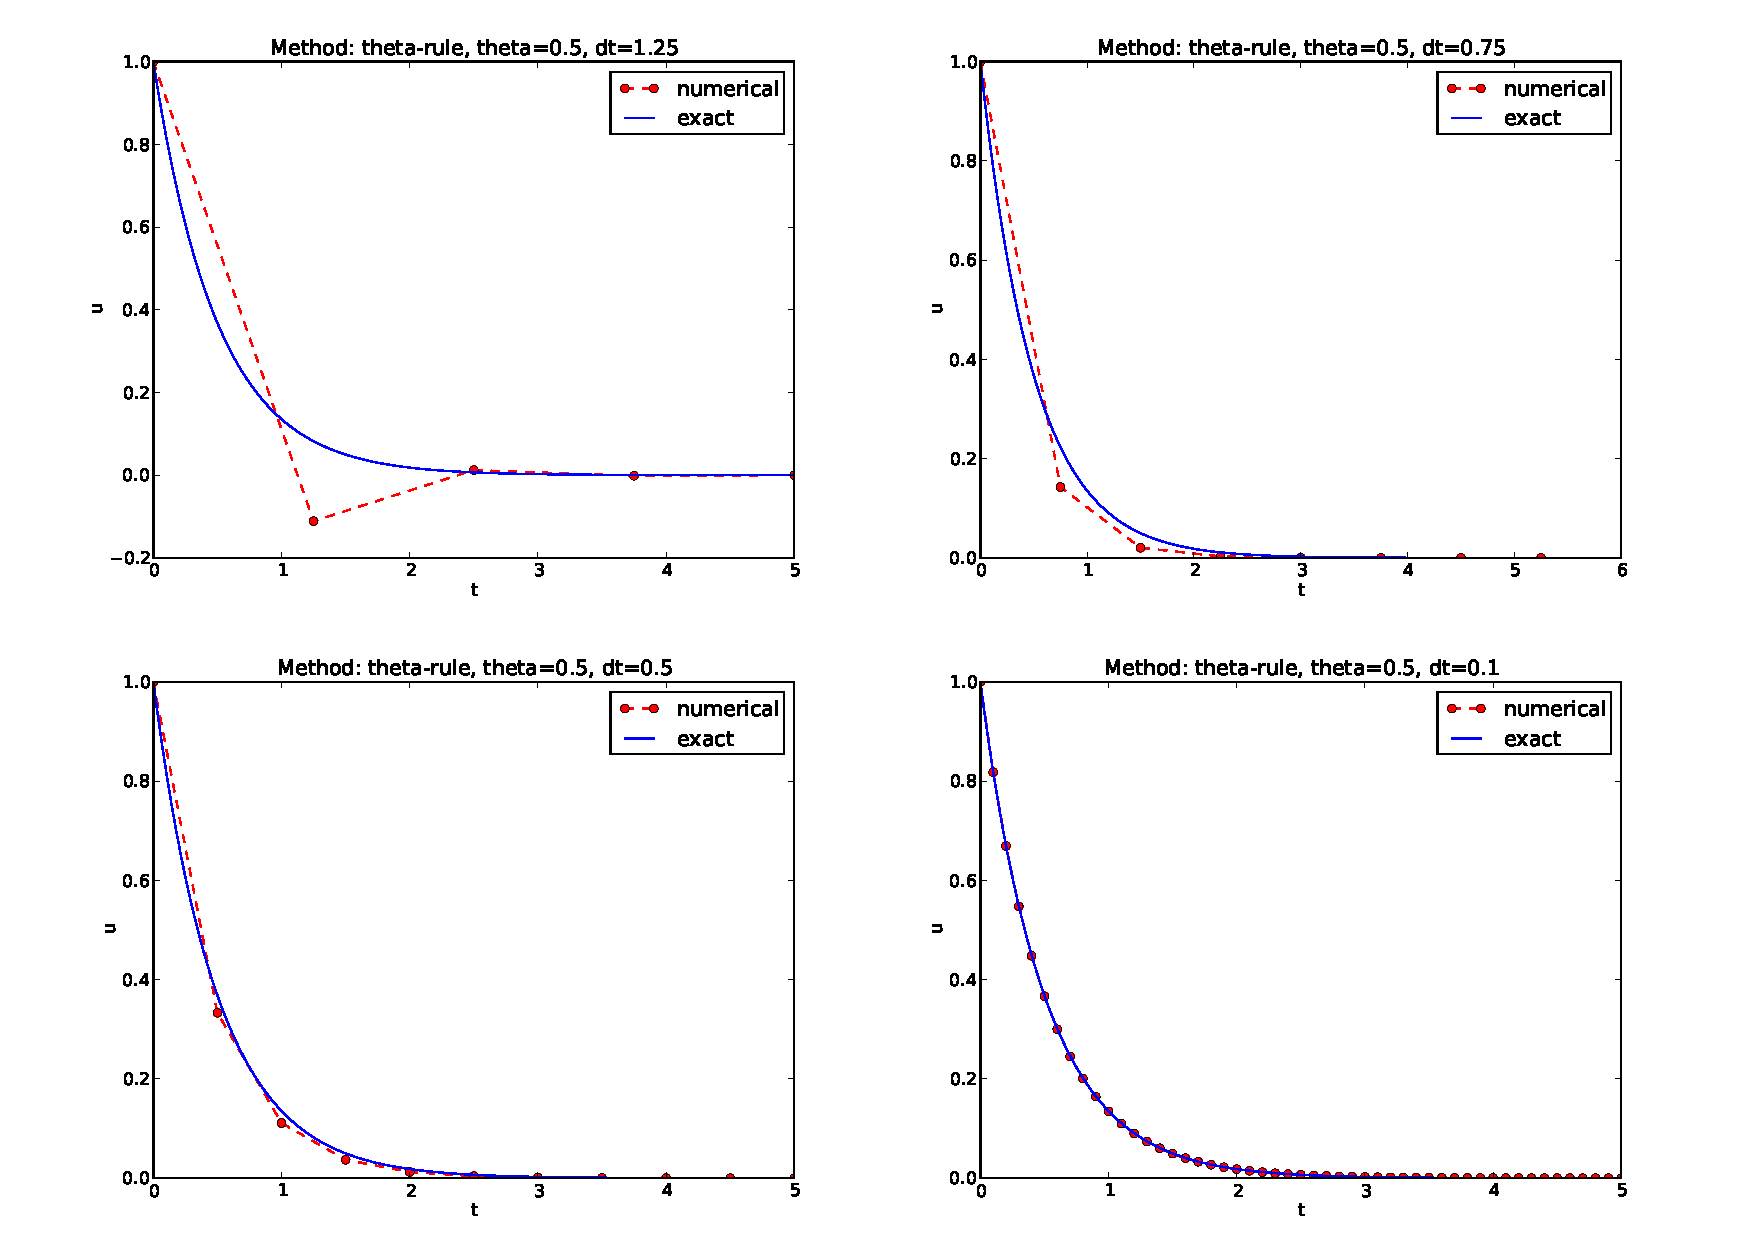
\includegraphics[width=1.1\linewidth]{fig-analysis/CN4c.pdf}}



\begin{itemize}
 \item $\Delta t=1.25$ and $A=-0.25$: oscillatory solution

 \item Never any growing solution
\end{itemize}

\noindent
\end{frame}

\begin{frame}[plain,fragile]
\frametitle{Summary of stability}

\begin{enumerate}
\item Forward Euler is \emph{conditionally stable}
\begin{itemize}

   \item $\Delta t < 2/a$ for avoiding growth

   \item $\Delta t\leq 1/a$ for avoiding oscillations

\end{itemize}

\noindent
\item The Crank-Nicolson is \emph{unconditionally stable} wrt growth
   and conditionally stable wrt oscillations
\begin{itemize}

   \item $\Delta t < 2/a$ for avoiding oscillations

\end{itemize}

\noindent
\item Backward Euler is unconditionally stable
\end{enumerate}

\noindent
\end{frame}

\begin{frame}[plain,fragile]
\frametitle{Comparing amplification factors}

$u^{n+1}$ is an amplification $A$ of $u^n$:

\[ u^{n+1} = Au^n,\quad A = \frac{1 - (1-\theta) a\Delta t}{1 + \theta a\Delta t} \]

The exact solution is also an amplification:

\[ u(t_{n+1}) = \Aex u(t_n), \quad \Aex = e^{-a\Delta t}\]

A possible measure of accuracy: $\Aex - A$
\end{frame}

\begin{frame}[plain,fragile]
\frametitle{Plot of amplification factors}

% inline figure
\centerline{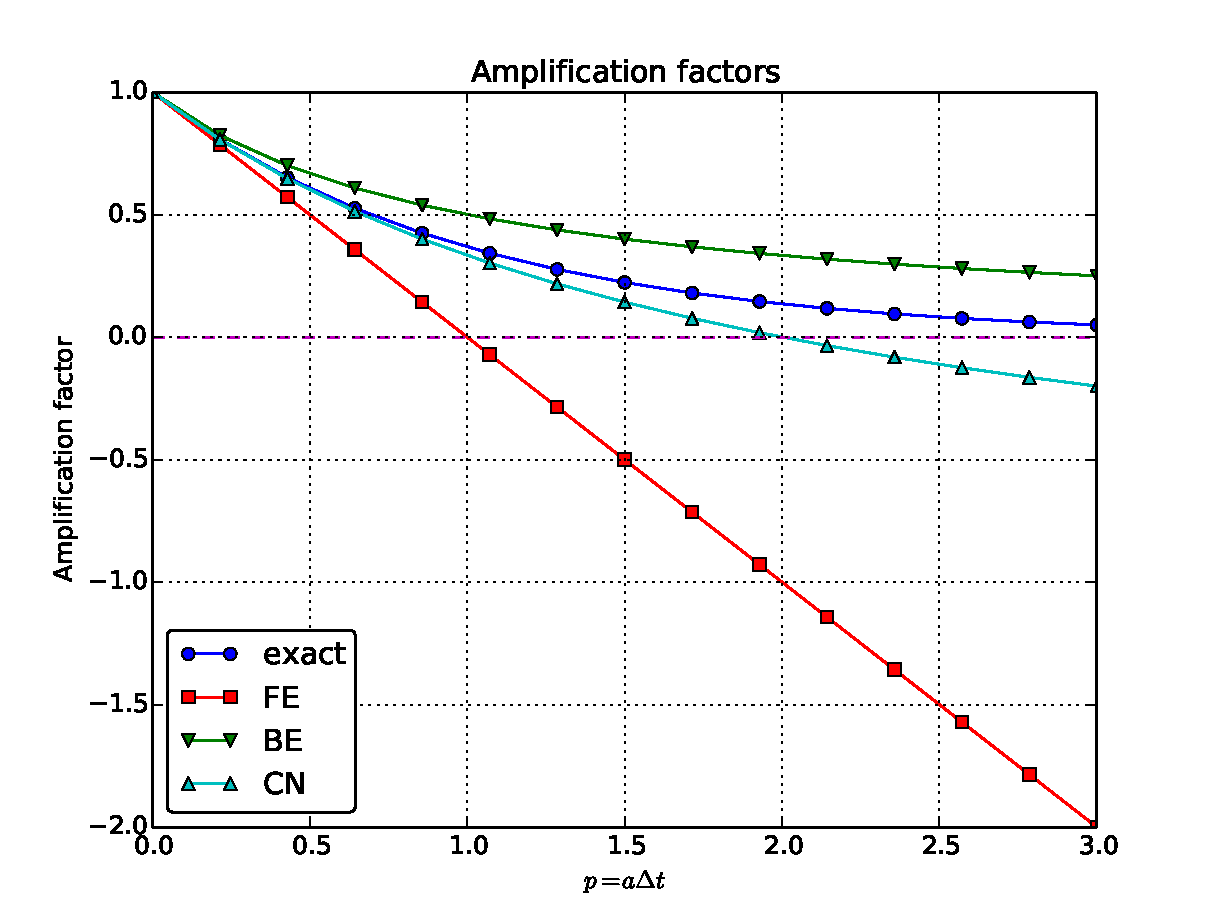
\includegraphics[width=0.9\linewidth]{fig-analysis/A_factors.pdf}}
\end{frame}

\begin{frame}[plain,fragile]
\frametitle{$p=a\Delta t$ is the important parameter for numerical performance}

\begin{itemize}
 \item $p=a\Delta t$ is a dimensionless parameter

 \item all expressions for stability and accuracy involve $p$

 \item Note that $\Delta t$ alone is not so important, it is the
   combination with $a$ through $p=a\Delta t$ that matters
\end{itemize}

\noindent
\begin{block}{Another ``proof'' why $p=a\Delta t$ is key }
If we scale the model
by $\bar t=at$, $\bar u=u/I$, we get
$d\bar u/d\bar t = -\bar u$, $\bar u(0)=1$ (no physical parameters!).
The analysis show that $\Delta \bar t$ is key, corresponding to
$a\Delta t$ in the unscaled model.
\end{block}
\end{frame}

\begin{frame}[plain,fragile]
\frametitle{Series expansion of amplification factors}

To investigate $\Aex - A$ mathematically, we
can Taylor expand the expression, using $p=a\Delta t$ as variable.

\begin{minted}[fontsize=\fontsize{9pt}{9pt},linenos=false,mathescape,baselinestretch=1.0,fontfamily=tt,xleftmargin=2mm]{ipy}
>>> from sympy import *
>>> # Create p as a mathematical symbol with name 'p'
>>> p = Symbol('p')
>>> # Create a mathematical expression with p
>>> A_e = exp(-p)
>>>
>>> # Find the first 6 terms of the Taylor series of A_e
>>> A_e.series(p, 0, 6)
1 + (1/2)*p**2 - p - 1/6*p**3 - 1/120*p**5 + (1/24)*p**4 + O(p**6)

>>> theta = Symbol('theta')
>>> A = (1-(1-theta)*p)/(1+theta*p)
>>> FE = A_e.series(p, 0, 4) - A.subs(theta, 0).series(p, 0, 4)
>>> BE = A_e.series(p, 0, 4) - A.subs(theta, 1).series(p, 0, 4)
>>> half = Rational(1,2)  # exact fraction 1/2
>>> CN = A_e.series(p, 0, 4) - A.subs(theta, half).series(p, 0, 4)
>>> FE
(1/2)*p**2 - 1/6*p**3 + O(p**4)
>>> BE
-1/2*p**2 + (5/6)*p**3 + O(p**4)
>>> CN
(1/12)*p**3 + O(p**4)
\end{minted}
\end{frame}

\begin{frame}[plain,fragile]
\frametitle{Error in amplification factors}

Focus: the error measure $A-\Aex$ as function of $\Delta t$ (recall that $p=a\Delta t$):

\begin{equation}
A-\Aex = \left\lbrace\begin{array}{ll}
\Oof{\Delta t^2}, & \hbox{Forward and Backward Euler},\\ 
\Oof{\Delta t^3}, & \hbox{Crank-Nicolson}
\end{array}\right.
\end{equation}
\end{frame}

\begin{frame}[plain,fragile]
\frametitle{The fraction of numerical and exact amplification factors}

Focus: the error measure $1-A/\Aex$ as function of $p=a\Delta t$:

\begin{minted}[fontsize=\fontsize{9pt}{9pt},linenos=false,mathescape,baselinestretch=1.0,fontfamily=tt,xleftmargin=2mm]{ipy}
>>> FE = 1 - (A.subs(theta, 0)/A_e).series(p, 0, 4)
>>> BE = 1 - (A.subs(theta, 1)/A_e).series(p, 0, 4)
>>> CN = 1 - (A.subs(theta, half)/A_e).series(p, 0, 4)
>>> FE
(1/2)*p**2 + (1/3)*p**3 + O(p**4)
>>> BE
-1/2*p**2 + (1/3)*p**3 + O(p**4)
>>> CN
(1/12)*p**3 + O(p**4)
\end{minted}
Same leading-order terms as for the error measure $A-\Aex$.
\end{frame}

\begin{frame}[plain,fragile]
\frametitle{The true/global error at a point}

\label{decay:analysis:gobal:error}

\begin{itemize}
 \item The error in $A$ reflects the \emph{local error} when going from one
   time step to the next

 \item What is the \emph{global (true) error} at $t_n$?
   $e^n = \uex(t_n) - u^n = Ie^{-at_n} - IA^n$

 \item Taylor series expansions of $e^n$ simplify the expression
\end{itemize}

\noindent
\end{frame}

\begin{frame}[plain,fragile]
\frametitle{Computing the global error at a point}

\begin{minted}[fontsize=\fontsize{9pt}{9pt},linenos=false,mathescape,baselinestretch=1.0,fontfamily=tt,xleftmargin=2mm]{ipy}
>>> n = Symbol('n')
>>> u_e = exp(-p*n)   # I=1
>>> u_n = A**n        # I=1
>>> FE = u_e.series(p, 0, 4) - u_n.subs(theta, 0).series(p, 0, 4)
>>> BE = u_e.series(p, 0, 4) - u_n.subs(theta, 1).series(p, 0, 4)
>>> CN = u_e.series(p, 0, 4) - u_n.subs(theta, half).series(p, 0, 4)
>>> FE
(1/2)*n*p**2 - 1/2*n**2*p**3 + (1/3)*n*p**3 + O(p**4)
>>> BE
(1/2)*n**2*p**3 - 1/2*n*p**2 + (1/3)*n*p**3 + O(p**4)
>>> CN
(1/12)*n*p**3 + O(p**4)
\end{minted}
Substitute $n$ by $t/\Delta t$:

\begin{itemize}
 \item Forward and Backward Euler: leading order term $\half ta^2\Delta t$

 \item Crank-Nicolson: leading order term $\frac{1}{12}ta^3\Delta t^2$
\end{itemize}

\noindent
\end{frame}

\begin{frame}[plain,fragile]
\frametitle{Convergence}

The numerical scheme is convergent if the global error
$e^n\rightarrow 0$ as $\Delta t\rightarrow 0$.
If the error has a leading order term $\Delta t^r$, the
convergence rate is of order $r$.
\end{frame}

\begin{frame}[plain,fragile]
\frametitle{Integrated errors}

Focus: norm of the numerical error

\[ ||e^n||_{\ell^2} = \sqrt{\Delta t\sum_{n=0}^{N_t} ({\uex}(t_n) - u^n)^2}\]

Forward and Backward Euler:

\[ ||e^n||_{\ell^2} = \frac{1}{4}\sqrt{\frac{T^3}{3}} a^2\Delta t\]

Crank-Nicolson:

\[ ||e^n||_{\ell^2} = \frac{1}{12}\sqrt{\frac{T^3}{3}}a^3\Delta t^2\]


\begin{block}{Summary of errors }
Analysis of both the pointwise and the time-integrated true errors:

\begin{itemize}
  \item 1st order for Forward and Backward Euler

  \item 2nd order for Crank-Nicolson
\end{itemize}

\noindent
\end{block}
\end{frame}

\begin{frame}[plain,fragile]
\frametitle{Truncation error}

\begin{itemize}
 \item How good is the discrete equation?

 \item Possible answer: see how well $\uex$ fits the discrete equation
\end{itemize}

\noindent
\[ \lbrack D_t u = -au\rbrack^n\]
i.e.,

\[ \frac{u^{n+1}-u^n}{\Delta t} = -au^n\]
Insert $\uex$ (which does not in general fulfill this equation):

\begin{equation}
\frac{\uex(t_{n+1})-\uex(t_n)}{\Delta t} + a\uex(t_n) = R^n \neq 0
\label{decay:analysis:trunc:Req}
\end{equation}
\end{frame}

\begin{frame}[plain,fragile]
\frametitle{Computation of the truncation error}

\begin{itemize}
 \item The residual $R^n$ is the \emph{truncation error}.

 \item How does $R^n$ vary with $\Delta t$?
\end{itemize}

\noindent
Tool: Taylor expand $\uex$ around the point where the ODE is sampled
(here $t_n$)


\[ \uex(t_{n+1}) = \uex(t_n) + \uex'(t_n)\Delta t + \half\uex''(t_n)
\Delta t^2 + \cdots \]
Inserting this Taylor series in (\ref{decay:analysis:trunc:Req}) gives

\[ R^n = \uex'(t_n) + \half\uex''(t_n)\Delta t + \ldots + a\uex(t_n)\]
Now, $\uex$ solves the ODE $\uex'=-a\uex$, and then

\[ R^n \approx \half\uex''(t_n)\Delta t\]
This is a mathematical expression for the truncation error.
\end{frame}

\begin{frame}[plain,fragile]
\frametitle{The truncation error for other schemes}

Backward Euler:

\[ R^n \approx -\half\uex''(t_n)\Delta t \]

Crank-Nicolson:

\[ R^{n+\half} \approx \frac{1}{24}\uex'''(t_{n+\half})\Delta t^2\]
\end{frame}

\begin{frame}[plain,fragile]
\frametitle{Consistency, stability, and convergence}

\index{consistency} \index{stability} \index{convergence}

\begin{itemize}
  \item Truncation error measures the residual in the difference equations.
    The scheme is \emph{consistent} if the truncation error goes to 0
    as $\Delta t\rightarrow 0$. Importance: the difference equations
    approaches the differential equation as $\Delta t\rightarrow 0$.

  \item \emph{Stability} means that the numerical solution exhibits the same
    qualitative properties as the exact solution. Here: monotone,
    decaying function.

  \item \emph{Convergence} implies that the true (global) error
    $e^n =\uex(t_n)-u^n\rightarrow 0$ as $\Delta t\rightarrow 0$.
    This is really what we want!
\end{itemize}

\noindent
The Lax equivalence theorem for \emph{linear} differential equations:
consistency + stability is equivalent with convergence.

(Consistency and stability is in most problems
much easier to establish than
convergence.)
\end{frame}

\end{document}
